\documentclass[12pt,a4paper]{article}
\usepackage[utf8]{inputenc}
\usepackage[spanish]{babel}
\usepackage{amsmath}
\usepackage{amsfonts}
\usepackage{amssymb}
\usepackage{makeidx}
\usepackage{graphicx}
\usepackage{lmodern}
\usepackage{kpfonts}
\usepackage{fourier}
\usepackage[left=2cm,right=2cm,top=2cm,bottom=2cm]{geometry}
\author{Joan Moran - Carolina González - Ronaldo Larrosa}


\title{Proyecto Segundo Parcial}
\maketitle Proyecto Segundo Parcial Proceso de Software 
\newpage
\tableofcontents
\newpage

\section{Normas ISO}

ISO (Organización Internacional de Normalización) es una federación mundial de organismos nacionales de normalización (organismos miembros de ISO). El trabajo de preparación de las normas internacionales normalmente se realiza a través de los comités técnicos de ISO. Cada organismo miembro interesado en una materia para la cual se haya establecido un comité técnico, tiene el derecho de estar representado en dicho comité. Las organizaciones internacionales, públicas y privadas, en coordinación con ISO, también participan en el trabajo. ISO colabora estrechamente con la Comisión Electrotécnica Internacional (IEC) en todas las materias de normalización electrotécnica.\\
\subsection{Norma ISO 9001}


La Norma ISO 9001 especifica los requisitos para un sistema de gestión de la calidad que pueden utilizarse para su aplicación interna por las organizaciones, para certificación o con fines contractuales. Se centra en la eficacia del sistema de gestión de la calidad para satisfacer los requisitos del cliente.\\

\section{Caso de Estudio}

Muzei es un fondo de pantalla en vivo que actualiza suavemente su pantalla de inicio cada día con famosas obras de arte. También retrocede hacia el fondo, difumina y atenúa las ilustraciones para mantener sus íconos y widgets en el centro de atención. Simplemente toque dos veces el fondo de pantalla o abra la aplicación Muzei para disfrutar y explorar la obra de arte en todo su esplendor.\\

Alternativamente, puede elegir sus fotos favoritas de su propia galería u otras aplicaciones para usar en su pantalla de inicio. Para mantener su fondo de pantalla fresco, Muzei rotará a través de sus fotos favoritas después de un determinado tiempo.\\

\begin{Imagen}
\centering
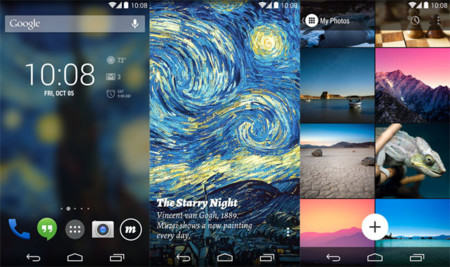
\includegraphics[scale=0.5]{Imagen.jpg}
\end{Imagen}


\section{Contexto del Proyecto}


Muzei es amigable para los desarrolladores. Todo el código está disponible en http://code.muzei.co y Muzei incluso ofrece una API simple que le permite crear su propia fuente de fondo de pantalla. Para detalles de API, visite http://api.muzei.co.\\

Si utiliza una Fuente heredada de terceros, debe desactivar las Optimizaciones de la batería en esa aplicación para permitir que continúe cargando las ilustraciones. Consulte https://medium.com/muzei/muzei-3-0-and-legacy-sources-8261979e2264 para obtener más detalles.\\


Muzei ahora incluye una carátula para Android Wear, ¡para que puedas ver tu último fondo de pantalla directamente en tu muñeca!\\


Hecho por Roman Nurik e Ian Lake, junto con las contribuciones de muchos en la comunidad de Android. Muzei es una transliteración de la palabra rusa музей, que significa "museo".\\

Las obras de arte destacadas en Muzei están a diario a cargo de nuestro reducido personal y son posibles gracias a WikiArt.org y sus colaboradores.\\


\subsection{Requerimientos}
a)	Es una aplicación que actualizará constantemente el fondo de pantalla del móvil.\\
b)	Disminuir la intensidad para mantener la visibilidad de los iconos.\\
c)	Android 4.2 o superior\\

\subsection{Diseño y Desarrollo}
Existe una infinidad de librerías, que ayudan en muchas ocasiones. Con ellas, se puede darle un toque profesional a la interfaz con alguna animación interesante, eliminar la necesidad de escribir líneas de código repetitivo, conectar una aplicación a Internet y realizar acciones REST con relativa facilidad. Las principales librerias utilizadas para la creación del presente proyecto proyecto son:\\
import android.os.Bundle\\
import android.view.View\\
import android.widget.Toast\\
import androidx.appcompat.widget.Toolbar\\
import androidx.core.content.edit\\
import androidx.fragment.app.Fragment\\
import androidx.fragment.app.FragmentManager\\
import com.google.android.apps.muzei.isPreviewMode\\
import com.google.android.apps.muzei.render.MuzeiBlurRenderer\\
import com.google.android.apps.muzei.util.toast\\
import com.google.android.material.tabs.TabLayout\\
import net.nurik.roman.muzei.R\\
import net.nurik.roman.muzei.databinding.EffectsFragmentBinding\\

Actualizar 'Examinar' solo a solicitud del usuario\\

Algunas fuentes reaccionan mal a las llamadas solicitadas por onLoad, por lo que se recomienda deshabilitar la actualización automática cuando vaya a la pantalla 'Examinar' y solo actualice las solicitudes específicas de los usuarios.\\
importar  androidx.lifecycle.switchMap\\
importar  androidx.lifecycle.viewModelScope\\
importar  com.google.android.apps.muzei.room.Artwork\\
importar  com.google.android.apps.muzei.sync.ProviderManager\\
importar  com.google.android.apps.muzei.util.ContentProviderClientCompat\\
importar  kotlinx.coroutines.CoroutineScope\\
importar  kotlinx.coroutines.asCoroutineDispatcher\\
@@ -102,9 +101,6 @@ clase BrowseProviderViewModel (\\

    fun  setContentUri ( contentUri :  Uri ) {\\
        contentUriLiveData.value = contentUri\\
        viewModelScope.launch {\\
            ProviderManager .requestLoad (getApplication (),\\ contentUri)\\
        }\\
    }\\

    val artLiveData :  LiveData < List < Artwork >> = contentUriLiveData.switchMap {contentUri - >
    
    
    
  
\subsection{API}
Paquete com.google.android.apps.muzei.api\\
Resumen de clase\\
Ilustraciones:	Un objeto serializable que representa una sola obra de arte producida por a MuzeiArtSource.\\
Artwork.Builder:	Una interfaz fluida estilo constructor para crear objetos.Artwork
MuzeiArtSource:	Clase base para una fuente de arte Muzei Live Wallpaper.\\
MuzeiContract:	Contrato para Muzei ContentProvider, permitiendo que otras aplicaciones lean los datos de arte actuales de Muzei.\\
MuzeiContract.Artwork:	Constantes y métodos auxiliares para la tabla Artwork, proporcionando acceso a la obra de arte actual.\\
RemoteMuzeiArtSource:	Una subclase de conveniencia MuzeiArtSourcediseñada específicamente para su uso por fuentes de arte que obtienen metadatos de ilustraciones de forma remota.\\
UserCommand:	Clase de datos que representa un comando visible para el usuario.\\


\subsection{Actualizar código de versión para Muzei 3.3.0 RC 1}
nombre = 3.3.0\\
# Número de versión + ID único para la compilación\\
codeWear = 330005\\
codeWear = 330007\\
# La aplicación principal debe ser exclusiva de la versión Wear\\
código = 330004\\
código = 330006\\

# Último número beta para esta versión. Solo se aplica a las versiones beta.\\
betaNumber = Beta 3\\
betaNumber = RC 1\\

\section{Interfaz}
La interfaz del proyecto es amigable con el usuario, puesto que es intuitiva y además de ser sencilla de manejar.\\

\begin{Interfaz}
\centering
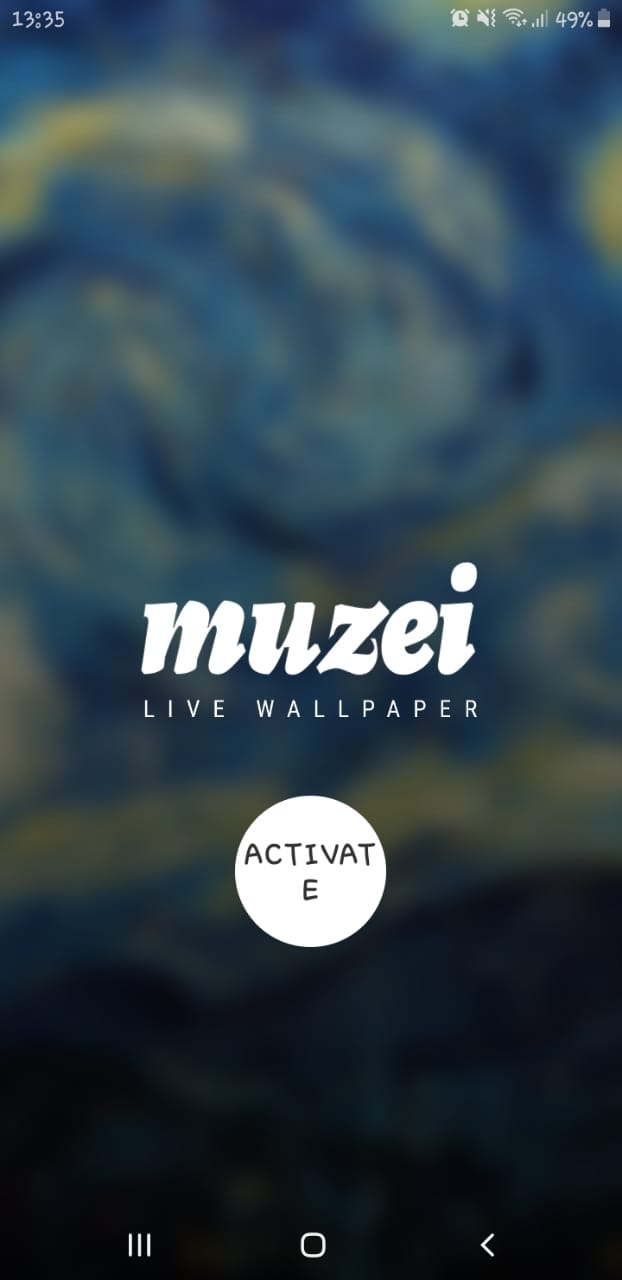
\includegraphics[scale=0.2]{Interfaz.jpeg}
\end{Interfaz}
\\
\\

\begin{prueba}
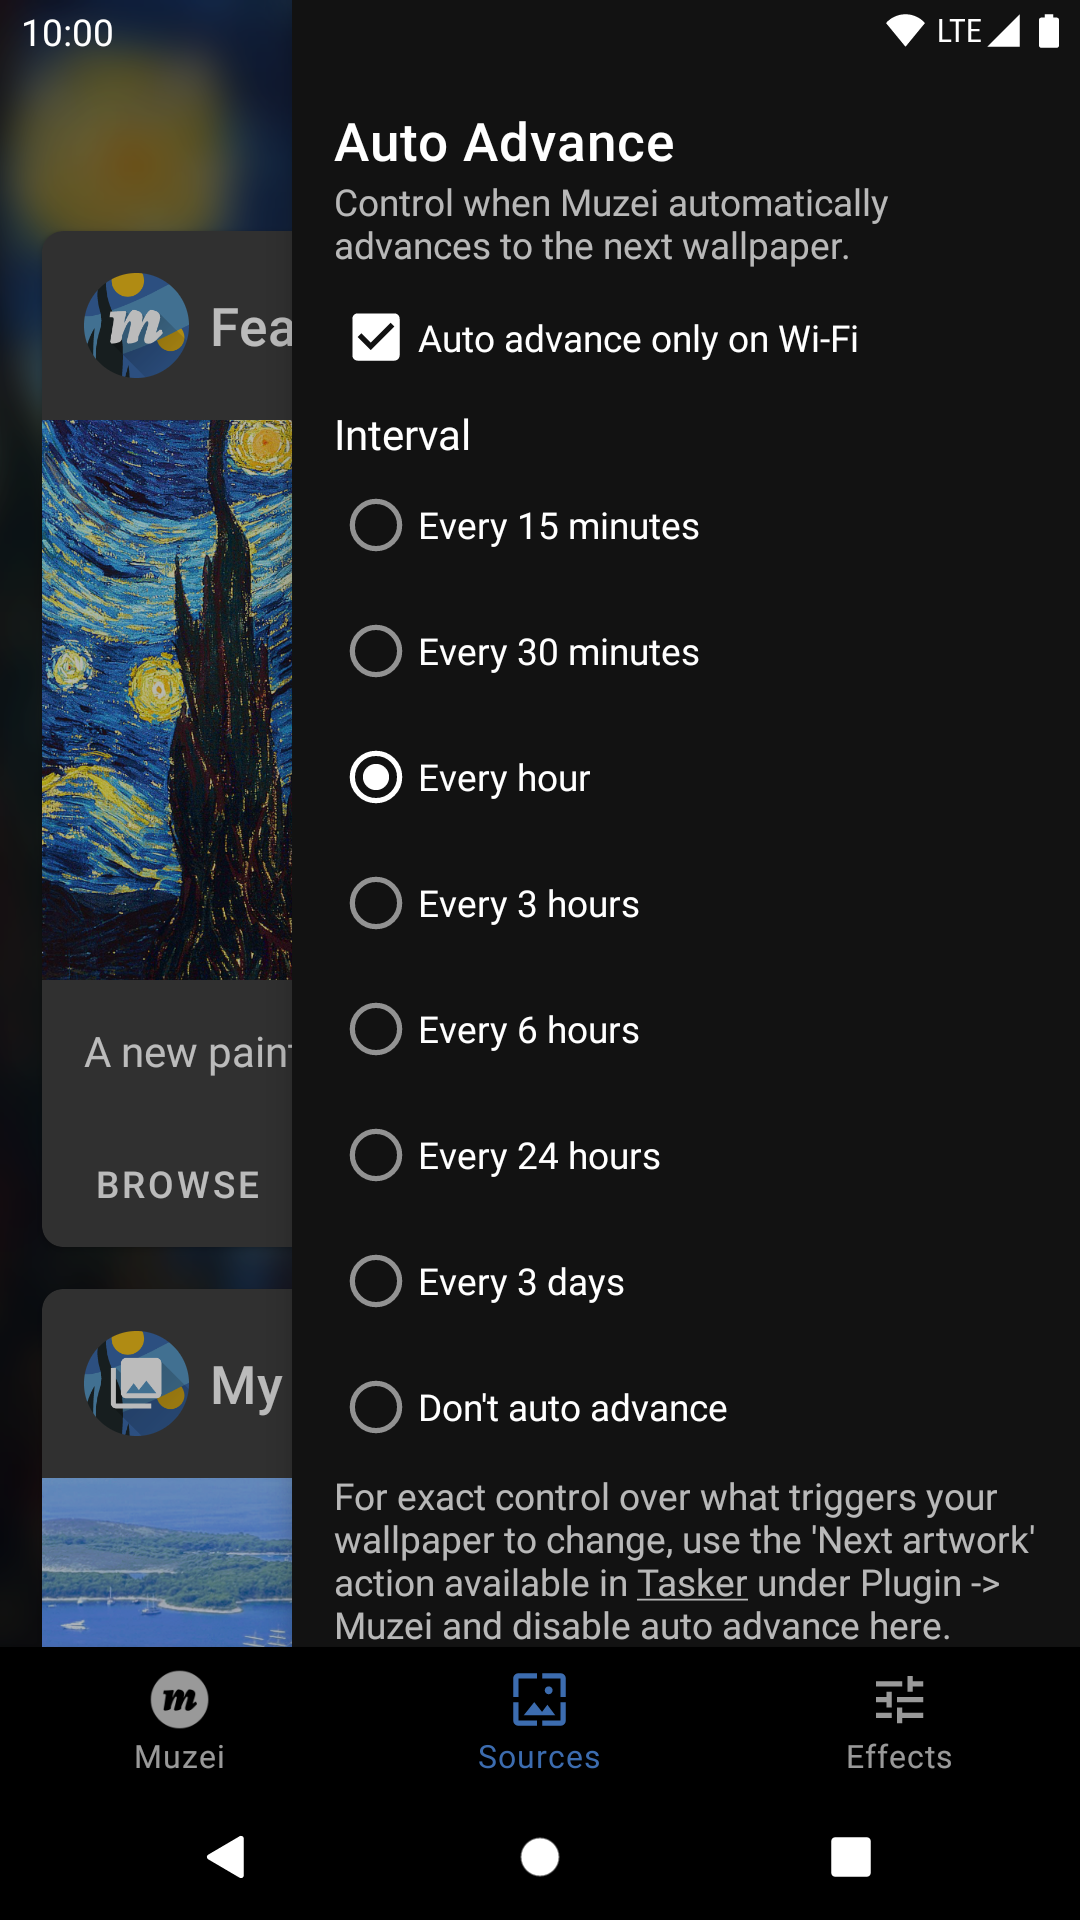
\includegraphics[scale=0.2]{prueba.png}
\end{prueba}

\section{Conclusión}
La organización debe mejorar continuamente la conveniencia, adecuación y eficacia del proyecto, puesto que de no hacerlo existiría la posibilidad de quedar obsoleto con el pasar del tiempo.

\section{Repositorio en GitHub}
Para el control de versiones del presente documento se utilizó la herramienta GitHub creando un repositorio compartido con los diferentes miembros del grupo el cual se encuentra en la siguiente dirección:  \\
https://github.com/joan2211/ProyectoSegundoParcial\\


\begin{Git}
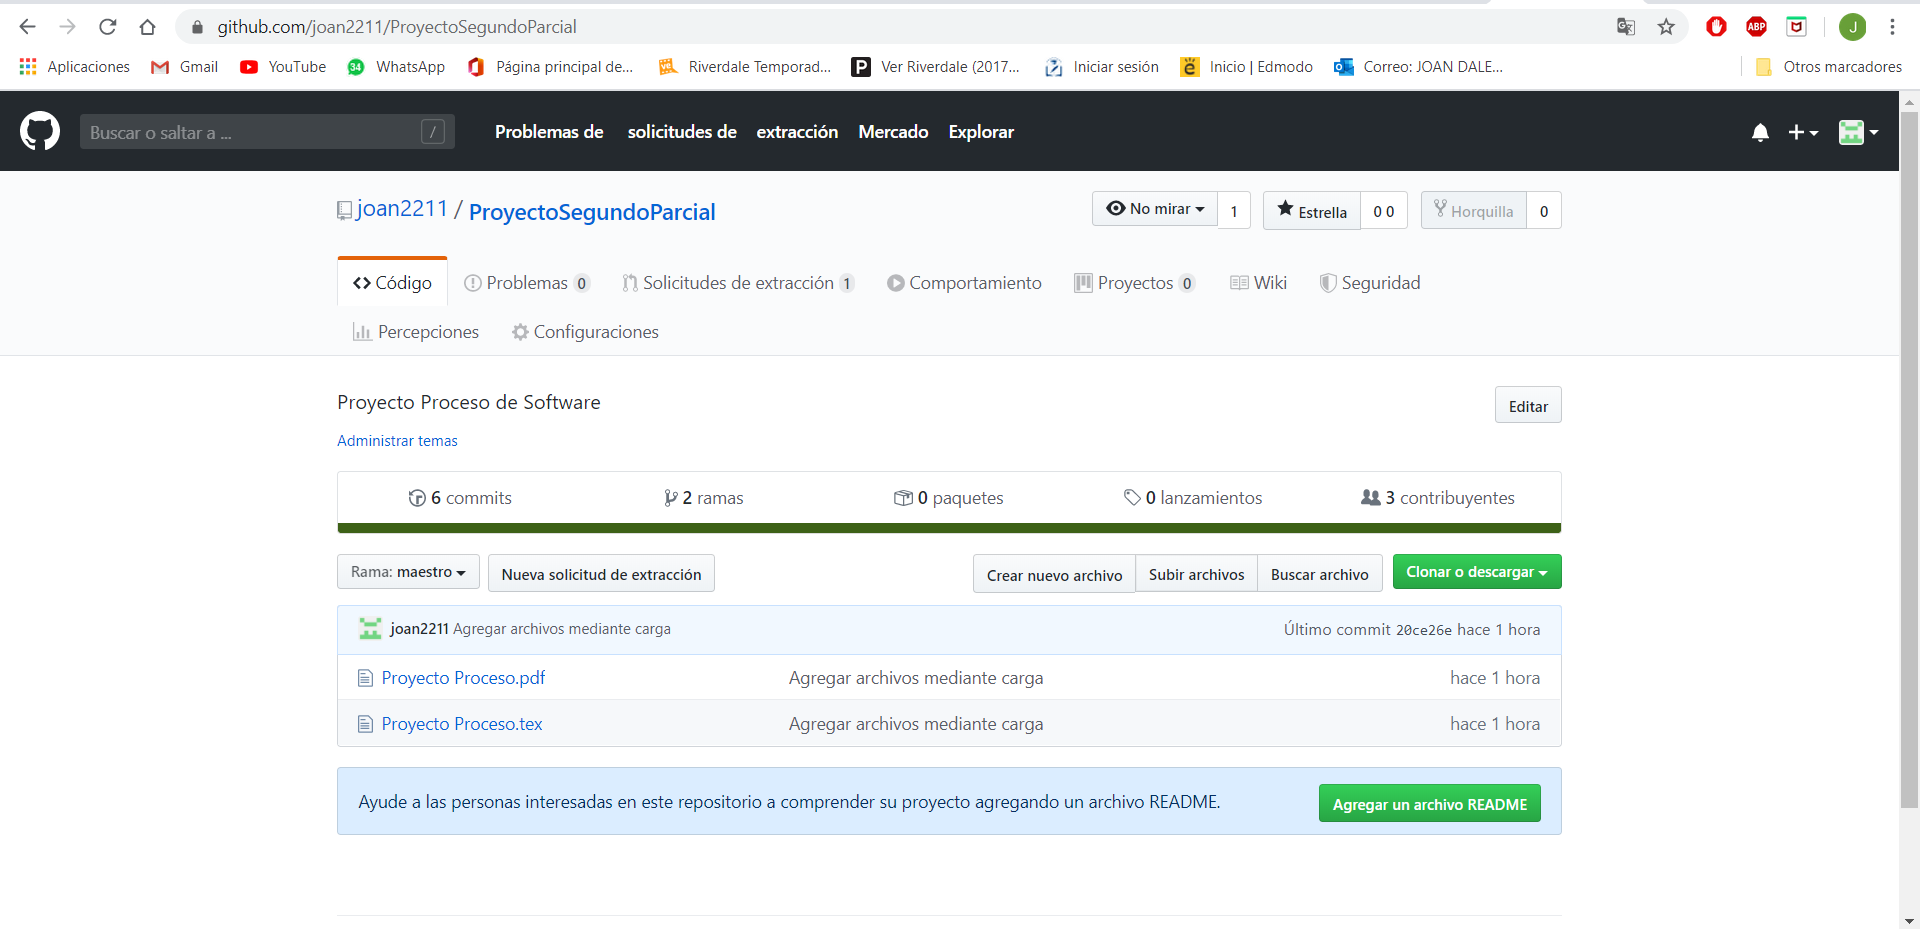
\includegraphics[scale=0.4]{GitHub.PNG}
\end{Git}

\end{document}
